
\cleardoublepage
\appendix
\renewcommand{\thechapter}{A}

\renewcommand{\thesection}{\Alph{chapter}.\arabic{section}}

\chapter{Mathematische Hintergründe und Herleitungen}
\label{anhangA}

In diesem Anhang werden die im Haupttext angesprochenen physikalischen Konzepte
formal und mathematisch vertieft. Ziel ist es, die didaktische Lesbarkeit der
Kapitel nicht zu beeinträchtigen und zugleich interessierten Lesern die
vollständigen Herleitungen zugänglich zu machen. 


%\section{Kapitel I}
\phantomsection
\section{Herleitung der Irrationalität der $\sqrt{2}$}
\label{anhangA_wurzel2}


\subsection*{Die Irrationalität von \texorpdfstring{$\sqrt{2}$}{sqrt(2)}}
\phantomsection

Der Beweis, dass $\sqrt{2}$ irrational ist, gehört zu den ältesten und
elegantesten Widerspruchsbeweisen \index{Widerspruchsbeweis}der Mathematik. 
Die Idee ist einfach: Wir nehmen an, dass $\sqrt{2}$ rational sei, und
zeigen dann, dass diese Annahme zu einem logischen Widerspruch führt.

\subsubsection*{Annahme}
\phantomsection
Wir nehmen an, dass $\sqrt{2}$ als vollständig gekürzter Bruch
\[
\sqrt{2} = \frac{p}{q},
\]
geschrieben werden kann, wobei $p$ und $q$ ganze Zahlen sind,
$q \neq 0$ und $p$ und $q$ teilerfremd sind.

\subsubsection*{Quadratbildung}
\phantomsection
Quadrieren beider Seiten ergibt
\[
2 = \frac{p^2}{q^2}
\qquad\Rightarrow\qquad
p^2 = 2q^2.
\]

Die rechte Seite ist gerade, also muss auch $p^2$ gerade sein.
Damit ist auch $p$ gerade. Es gibt also eine ganze Zahl $r$ mit
\[
p = 2r.
\]

\subsubsection*{Einsetzen und erneuter Schluss}
\phantomsection
Setzen wir dies in die Gleichung $p^2 = 2q^2$ ein, erhalten wir
\[
(2r)^2 = 2q^2,
\]
also
\[
4r^2 = 2q^2.
\]

Teilen durch $2$ liefert
\[
2r^2 = q^2.
\]

Also ist auch $q^2$ gerade – und damit $q$ selbst gerade.

\subsubsection*{Der Widerspruch}
\phantomsection
\index{Widerspruch}
Wir haben nun gezeigt:
\[
p \text{ ist gerade}, \qquad q \text{ ist gerade}.
\]
Damit besitzen $p$ und $q$ einen gemeinsamen Faktor $2$ und sind nicht
teilerfremd.

Das widerspricht unserer Ausgangsannahme, dass $\frac{p}{q}$ vollständig
gekürzt ist.

\subsubsection*{Folgerung}
Die Annahme, $\sqrt{2}$ sei rational, führt zum Widerspruch. Daher muss
\[
\sqrt{2} \text{ irrational sein.}
\]

Dieser klassische Beweis geht in seinen Grundzügen bereits auf Euklid\index{Euklid}
zurück und zeigt eindrucksvoll, wie Widerspruchsbeweise funktionieren.



\begin{DidacticBox}[Warum dieser Beweis so elegant ist]
	Der Beweis für die Irrationalität von $\sqrt{2}$ ist ein klassisches
	Beispiel dafür, wie mächtig Widerspruchsbeweise sein können. 
	Aus einer scheinbar harmlosen Annahme folgt eine logische Unmöglichkeit.
	Damit zeigt der Beweis nicht nur, dass $\sqrt{2}$ irrational ist, 
	sondern auch, wie präzise mathematisches Denken funktioniert.
\end{DidacticBox}




\section{Konstruktion der komplexen Zahlen}\index{komplexe Zahlen}
\label{anhangA_komplexe}
%\subsection*{A.2 Konstruktion der komplexen Zahl}
\phantomsection
\index{komplexe Zahlen}
Die Notwendigkeit komplexer Zahlen ergibt sich aus einem einfachen
Problem: Manche Gleichungen besitzen in den reellen Zahlen keine Lösung.
Das deutlichste Beispiel ist
\[
x^2 + 1 = 0.
\]

Durch Umformen erhält man
\[
x^2 = -1.
\]

Doch keine reelle Zahl besitzt ein negatives Quadrat. Damit zeigt sich
eine Grenze des reellen Zahlensystems. Trotzdem treten solche Ausdrücke
beim Lösen bestimmter Gleichungen – etwa im \emph{casus irreducibilis}\index{casus irreducibilis}
kubischer Gleichungen – zwangsläufig auf.

\subsubsection*{Ein neuer Zahlentyp}
\phantomsection
Um die Gleichung $x^2 = -1$ lösbar zu machen, führt man eine neue Zahl
ein und definiert
\[
i := \sqrt{-1}.
\]
\index{imaginäre Einheit $i$}
Diese Definition ist kein Trick, sondern eine Erweiterung des
Zahlensystems: Wir ergänzen die reellen Zahlen so, dass auch Gleichungen
mit negativen Quadraten sinnvoll lösbar werden.

\subsubsection*{Der Aufbau des neuen Zahlentyps}
\phantomsection
Jede Zahl der Form
\[
a + bi, \qquad a,b \in \mathbb{R},
\]
\index{komplexe Zahl $a+bi$}
heißt \emph{komplexe Zahl}. Die bekannten Rechenregeln bleiben gültig;
die einzige neue Information ist
\[
i^2 = -1.
\]

Daraus lassen sich Addition und Multiplikation vollständig bestimmen.
Ein Beispiel:
\[
(2 + 3i)(4 - i)
= 8 - 2i + 12i - 3i^2
= 11 + 10i.
\]

\begin{DidacticBox}[Warum die Einführung von $i$ notwendig ist]
	Die Zahl $i$ wird nicht eingeführt, weil man sie „erfinden“ wollte.
	Sie entsteht aus der inneren Logik der Algebra. Sobald man die
	Rechenregeln für Gleichungen akzeptiert, erzwingt die Gleichung
	$x^2 = -1$ die Einführung eines neuen Zahlentyps. 
	
	Alle komplexen Zahlen folgen dann aus der minimalen Annahme
	$i^2 = -1$. Damit wird das Zahlensystem abgeschlossen: Jedes Polynom
	besitzt nun mindestens eine Lösung (Fundamentalsatz der Algebra).\index{Fundamentalsatz der Algebra}
\end{DidacticBox}
\subsubsection*{Die Euler-Formel als geometrische Ergänzung}
\index{Euler-Formel}
\phantomsection
Die Einführung der Zahl $i$ erschließt nicht nur einen neuen Zahlenbereich,
sondern verbindet auch die Exponentialfunktion mit Kreisbewegungen.
Dies zeigt sich in der berühmten Euler-Formel
\[
e^{i\varphi} = \cos\varphi + i\sin\varphi.
\]
\subsubsection*{Kurze Herleitung der Euler-Formel mit Taylor-Reihen}
\phantomsection
\index{Taylor-Reihe}
Die Euler-Formel
\[
e^{i\varphi} = \cos\varphi + i\sin\varphi
\]
lässt sich elegant mit Potenzreihen (Taylor-Reihen) herleiten.

Zunächst betrachten wir die Reihenentwicklungen der Funktionen
$e^x$, $\cos x$ und $\sin x$ um den Punkt $x=0$:
\begin{align*}
	e^x &= 1 + x + \frac{x^2}{2!} + \frac{x^3}{3!} + \frac{x^4}{4!} + \cdots,\\[1ex]
	\cos x &= 1 - \frac{x^2}{2!} + \frac{x^4}{4!} - \frac{x^6}{6!} + \cdots,\\[1ex]
	\sin x &= x - \frac{x^3}{3!} + \frac{x^5}{5!} - \frac{x^7}{7!} + \cdots.
\end{align*}

Setzen wir nun in die Exponentialreihe $x = i\varphi$ ein, so erhalten wir
\[
e^{i\varphi} = 1 + i\varphi + \frac{(i\varphi)^2}{2!}
+ \frac{(i\varphi)^3}{3!}
+ \frac{(i\varphi)^4}{4!}
+ \cdots.
\]

Mit den Potenzen von $i$,
\[
i^2 = -1,\quad i^3 = -i,\quad i^4 = 1,\quad i^5 = i,\;\dots,
\]
können wir die Terme sortieren. Wir trennen Real- und Imaginärteil:

\begin{align*}
	e^{i\varphi}
	&= \Bigl(1 - \frac{\varphi^2}{2!} + \frac{\varphi^4}{4!} - \frac{\varphi^6}{6!} + \cdots\Bigr)
	\;+\; i\Bigl(\varphi - \frac{\varphi^3}{3!} + \frac{\varphi^5}{5!} - \frac{\varphi^7}{7!} + \cdots\Bigr)\\[1ex]
	&= \cos\varphi + i\sin\varphi.
\end{align*}

Damit ist die Euler-Formel
\[
e^{i\varphi} = \cos\varphi + i\sin\varphi
\]
als direkte Folge der Reihenentwicklungen von Exponential-, Sinus- 
und Kosinusfunktion hergeleitet.

\subsubsection*{Geometrische Idee}
\phantomsection
Betrachtet man die komplexe Ebene, so beschreibt ein Punkt auf dem
Einheitskreis \index{Einheitskreis} einen Winkel $\varphi$ zur reellen Achse.
Die Projektion auf die beiden Achsen ergibt
\[
(\cos\varphi,\;\sin\varphi).
\]
\index{Sinus}
\index{Kosinus}
Da die imaginäre Achse als Vielfaches von $i$ interpretiert wird,
entspricht dieser Punkt der komplexen Zahl
\[
\cos\varphi + i\sin\varphi.
\]

Die Euler-Formel zeigt, dass die komplexe Exponentialfunktion
genau diese Kreisbewegung beschreibt.

\begin{center}
	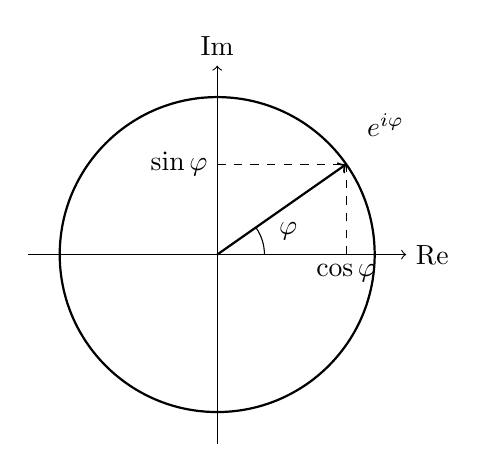
\begin{tikzpicture}[scale=2]
		% Kreis
		\draw[thick] (0,0) circle (1);
		% Achsen
		\draw[->] (-1.2,0) -- (1.2,0) node[right] {Re};
		\draw[->] (0,-1.2) -- (0,1.2) node[above] {Im};
		% Winkel
		\draw[thick,->] (0,0) -- ({cos(35)},{sin(35)});
		\draw (0.3,0) arc (0:35:0.3);
		\node at (0.45,0.15) {$\varphi$};
		% Projektionen
		\draw[dashed] ({cos(35)},0) -- ({cos(35)},{sin(35)});
		\draw[dashed] (0,{sin(35)}) -- ({cos(35)},{sin(35)});
		% Beschriftungen
		\node[below] at ({cos(35)},0) {$\cos\varphi$};
		\node[left] at (0,{sin(35)}) {$\sin\varphi$};
		\node at ({cos(35)+0.25},{sin(35)+0.25}) {$e^{i\varphi}$};
	\end{tikzpicture}
\end{center}

\subsubsection*{Multiplikation mit \boldmath$i$ als Drehung}
\phantomsection
\index{Drehung (Multiplikation mit $i$)}
In der komplexen Ebene hat die Multiplikation mit $i$ eine einfache geometrische 
Bedeutung: Sie dreht jede Zahl um $90^\circ$ gegen den Uhrzeigersinn.

Beispiele:
\[
1 \xrightarrow{\;\cdot i\;} i \xrightarrow{\;\cdot i\;} -1 
\xrightarrow{\;\cdot i\;} -i \xrightarrow{\;\cdot i\;} 1
\]

Jede weitere Multiplikation mit $i$ fügt eine weitere Drehung von $90^\circ$ hinzu.  
Wichtig: Die Länge (der Betrag) ändert sich dabei nicht – nur die Richtung.

Die Exponentialfunktion $e^{i\varphi}$ kombiniert unendlich viele solcher 
kleinen Drehungen. Dadurch entsteht eine kontinuierliche Rotation auf dem 
Einheitskreis, deren Winkel genau $\varphi$ beträgt.
\subsubsection*{Warum Multiplikation mit \boldmath$i$ eine Drehung erzeugt}
\phantomsection
Betrachten wir einen Punkt auf dem Einheitskreis:
\[
e^{i\varphi} = \cos\varphi + i\sin\varphi.
\]

Multiplizieren wir diesen Punkt mit $i$, so erhalten wir
\[
i \cdot e^{i\varphi}
= i(\cos\varphi + i\sin\varphi)
= i\cos\varphi - \sin\varphi.
\]

Dies entspricht der neuen komplexen Zahl
\[
-\sin\varphi + i\cos\varphi.
\]

Genau das erhält man auch, wenn man den ursprünglichen Punkt
\((\cos\varphi,\;\sin\varphi)\)
um \(90^\circ\) gegen den Uhrzeigersinn dreht:
\[
(\cos\varphi,\;\sin\varphi)
\;\longrightarrow\;
(-\sin\varphi,\;\cos\varphi).
\]

Damit ist klar:  
\[
i \cdot e^{i\varphi}
\]
ist \emph{genau} der Punkt, der um \(90^\circ\) gedreht wurde – bei unverändertem Radius.

\begin{DidacticBox}[Kernidee der Euler-Formel]
	Multiplikation mit $i$ bedeutet eine Drehung um $90^\circ$ in der komplexen Ebene.  
	Die Exponentialfunktion $e^{i\varphi}$ kombiniert viele solcher kleinen Drehungen 
	zu einer einzigen Rotation um den Winkel $\varphi$.
	
	Darum gilt:
	\[
	e^{i\varphi} = \cos\varphi + i\sin\varphi.
	\]
\end{DidacticBox}

\subsubsection*{Abschluss}
\phantomsection
Die komplexen Zahlen erweitern die reellen Zahlen um genau das, was
fehlt, um alle Gleichungen lösbar zu machen. Aus der einzelnen
Definition $i^2=-1$ entsteht ein vollständiger Zahlenbereich mit klaren
Regeln und einer geometrischen Struktur.
%============================================================
\section{Mandelbrot-Landkarte: mathematische Erzeugung und Farbgebung}
\label{app:mandelbrot-rendering}

\index{Mandelbrotmenge}
\index{Iteration}
\index{Escape-Radius}
\index{Fluchtzeit}
\index{Parameterraum}
\index{komplexe Ebene}
\index{Farbgebung}
\index{Algorithmus}

\textbf{Ziel dieses Anhangs:} Hier wird gezeigt, wie eine typische Mandelbrot-Grafik algorithmisch entsteht:
vom Bildpixel über den Parameter \(c\) bis zur Fluchtzeit und zur Farbzuordnung.

\begin{MathBox}[Grundprinzip: Pixel \(\rightarrow\) Parameter \(c\) \(\rightarrow\) Iteration]
	Wir berechnen für jeden Bildpunkt einen Parameter \(c\in\mathbb{C}\) und iterieren
	\[
	z_{n+1}=z_n^2+c,\qquad z_0=0.
	\]
	Die Mandelbrotmenge ist die Menge der Parameter \(c\), für die die Folge \(\{z_n\}\) beschränkt bleibt.
\end{MathBox}

%------------------------------------------------------------
\subsection*{Koordinatentransformation: vom Pixel in die komplexe Ebene}
\index{Koordinatentransformation}

Ein Bild habe Breite \(W\) und Höhe \(H\). Wir wählen ein Sichtfenster
\[
x\in[x_{\min},x_{\max}],\qquad y\in[y_{\min},y_{\max}]
\]
und ordnen jedem Pixel \((i,j)\) (mit \(0\le i<W\), \(0\le j<H\)) einen Parameter \(c=x+iy\) zu:
\[
x(i)=x_{\min}+\frac{i}{W-1}\,(x_{\max}-x_{\min}),\qquad
y(j)=y_{\max}-\frac{j}{H-1}\,(y_{\max}-y_{\min}),
\]
\[
c(i,j)=x(i)+i\,y(j).
\]
Das Minuszeichen bei \(y(j)\) kommt daher, dass Bildkoordinaten typischerweise nach unten wachsen.

\begin{NoteBox}[Typisches Standardfenster]
	Ein häufig verwendetes Fenster ist
	\[
	x\in[-2.5,1.0],\qquad y\in[-1.2,1.2].
	\]
	Für Details (Zoom) wählt man ein kleineres Fenster um ein Zentrum \(c_0\).
\end{NoteBox}

%------------------------------------------------------------
\subsection*{Escape-Time-Algorithmus: Fluchtkriterium und Iterationszahl}
\index{Fluchtkriterium}

Für jedes \(c\) iterieren wir bis zu einer Maximalzahl \(N_{\max}\). Sobald \(|z_n|>R\) gilt, stoppen wir.
Für die Mandelbrotiteration reicht klassisch \(R=2\):

\begin{MathBox}[Escape-Radius \(R=2\)]
	Für \(z_{n+1}=z_n^2+c\) gilt: Wenn für ein \(n\) \(|z_n|>2\), dann divergiert die Folge sicher.
\end{MathBox}

Formal definieren wir die \textbf{Fluchtzeit}
\[
n_\text{esc}(c)=\min\{n\in\mathbb{N}\mid |z_n|>2\},
\]
falls sie existiert; andernfalls setzen wir \(n_\text{esc}(c)=N_{\max}\) und markieren den Punkt als „innen“ (typisch schwarz).

%------------------------------------------------------------
\subsection*{Farbgebung: diskret, glatt und „schön“}
\index{Farbskala}

\subsubsection*{(a) Diskrete Farbgebung über Fluchtzeit}
Die einfachste Methode: ordne die Farbe nur nach \(n_\text{esc}\) zu.
Das führt oft zu sichtbaren „Bändern“ (Banding), ist aber didaktisch klar.

\subsubsection*{(b) Glatte Farbgebung (Continuous Coloring)}
Um Banding zu vermeiden, nutzt man eine \textbf{kontinuierliche} Iterationszahl. Eine verbreitete Variante ist:
\[
\nu(c)=n + 1 - \log_2\!\bigl(\log |z_n|\bigr),
\]
wobei \(n\) der erste Index ist mit \(|z_n|>2\). (Hier ist \(z_n\) bereits außerhalb; \(\nu\) liegt zwischen \(n\) und \(n+1\).)

\begin{DidacticBox}[Warum diese „Log-Log“-Formel?]
	Außerhalb wächst \(|z_n|\) ungefähr quadratisch. Durch \(\log(\log(\cdot))\) wird dieses Wachstum „linearisiert“,
	sodass Farbverläufe glatt werden und die Struktur am Rand deutlich besser sichtbar ist.
\end{DidacticBox}

Aus \(\nu\) macht man dann eine Zahl \(t\in[0,1]\) (z.B. durch Skalierung) und führt \(t\) durch eine Farbpalette.

\subsubsection*{(c) Histogramm-Equalization (optional, für sehr gleichmäßige Kontraste)}
Fortgeschritten: man zählt, wie viele Pixel welche Fluchtzeit haben, bildet eine kumulative Verteilung und verteilt Farben so,
dass häufige Werte nicht „zusammenkleben“. Das liefert sehr ausgewogene Bilder, ist aber reiner Rendering-Komfort.

%------------------------------------------------------------
\subsection*{Pseudocode: kompakt und nachvollziehbar}
\index{Pseudocode}

% Wenn du listings nutzt:
% \usepackage{listings}

\begin{verbatim}
	Input: W,H, x_min,x_max, y_min,y_max, N_max, R=2
	for j = 0..H-1:
	y = y_max - j*(y_max-y_min)/(H-1)
	for i = 0..W-1:
	x = x_min + i*(x_max-x_min)/(W-1)
	c = x + I*y
	z = 0
	n = 0
	while n < N_max and |z| <= R:
	z = z*z + c
	n = n + 1
	if n == N_max:
	color(i,j) = black   // inside (bounded up to N_max)
	else:
	// smooth iteration count (optional):
	nu = n + 1 - log2(log(|z|))
	color(i,j) = palette(nu)
	Output: PNG image
\end{verbatim}

\begin{NoteBox}[Wichtig für den Leser]
	Die Mandelbrotmenge selbst ist \emph{mathematisch} nur „innen vs. außen“ (beschränkt vs. divergent).
	Alles, was danach kommt (Palette, Glättung, Histogramm), ist \textbf{Darstellungstechnik}.
\end{NoteBox}

%============================================================